\chapter{Evaluation and Findings}



\section{Testing my implementation}
In order to keep tests fair, it is important to keep as much of the environment constant as possible between test iterations. Each iteration should have one variable that is changed so that the effects of this change can be easily observed and analysed. I have decied to investigate how changing the volume of traffic that is sent between client on a consumer network, effects the jitter with which the messages arrive.

The test is set up using the client hosted model where the clients are connected to the network on both an ethernet connection and WiFi. The host is connected to the router over ethernet cables that go through a switch. One client that will connect to the host is started on the same machine as the server; I will refer to this client as the ``localhost client''. Another client is connected directly to the router and I will refer to this one as ``ethernet client''. The last client that will connect to the host, is a laptop that is close to the router and connected over WiFi, this will be refered to as the ``WiFi client''.

Once the connection has been established, the server tickrate can be configured. This will be the variable that I will change and observe the effects of at each stage of the experiment.

\section{The results}

\subsection{Jitter between WiFi and Ethernet connections}



\begin{figure}[p]
  \centering
  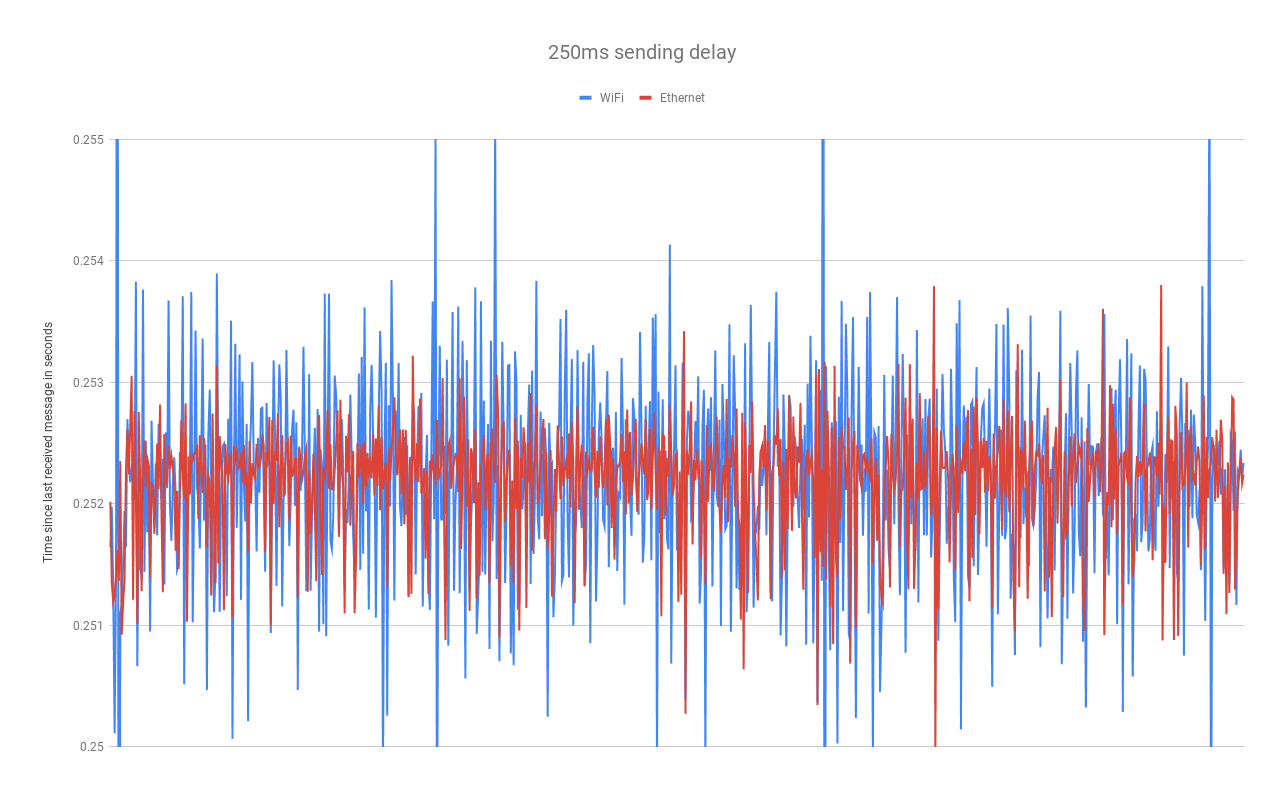
\includegraphics[width=\textwidth]{Graphs/250ms_delay}
  \caption{250ms Delay}
  \label{fig:250ms_graph}
\end{figure}

\begin{figure}[p]
  \centering
  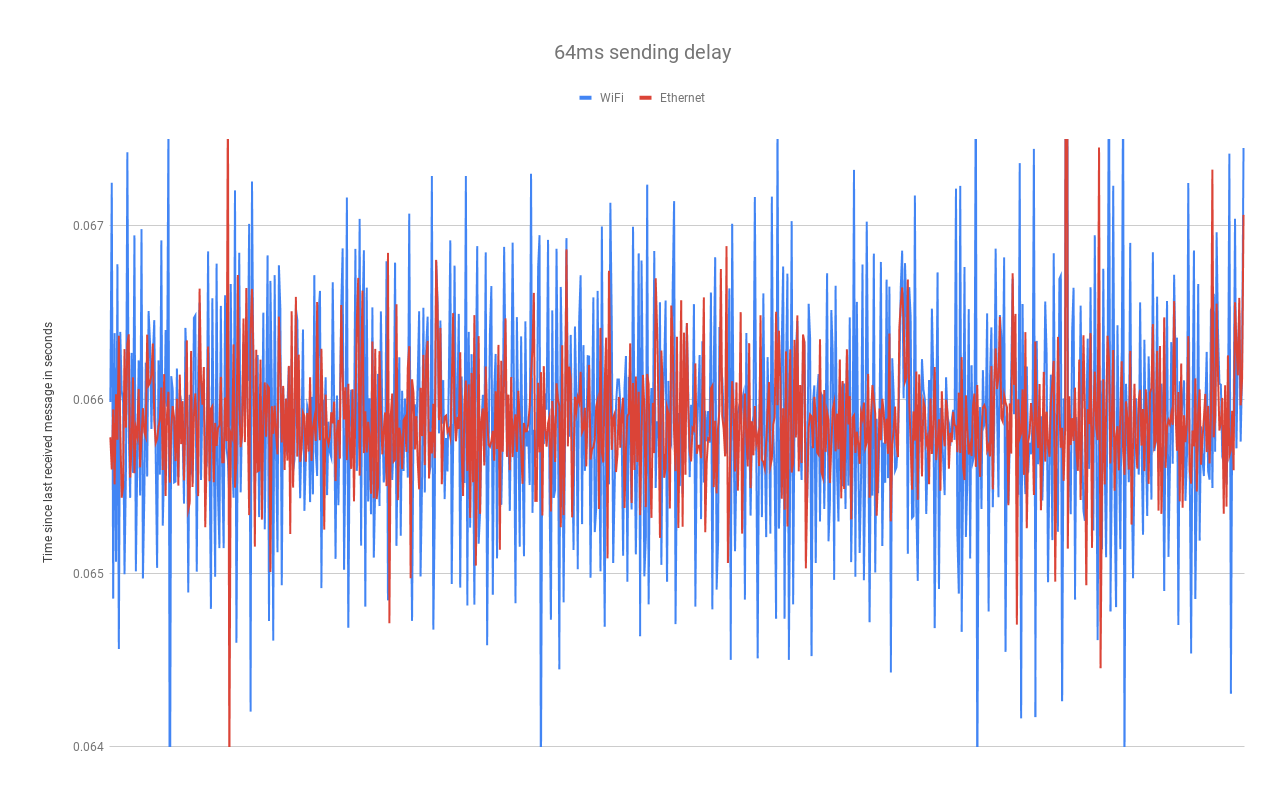
\includegraphics[width=\textwidth]{Graphs/64ms_delay}
  \caption{64ms Delay}
  \label{fig:64ms_graph}
\end{figure}

\begin{figure}[p]
  \centering
  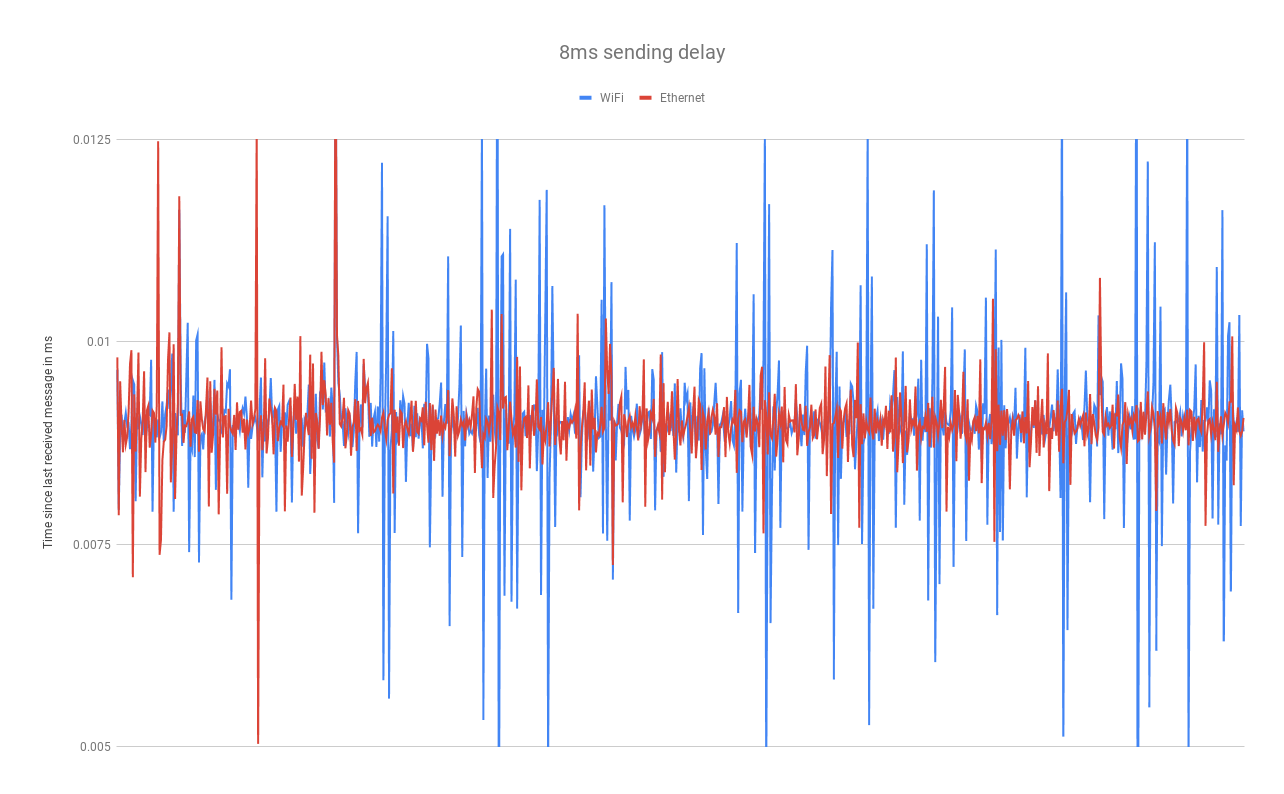
\includegraphics[width=\textwidth]{Graphs/8ms_delay}
  \caption{8ms Delay}
  \label{fig:8ms_graph}
\end{figure}



\subsection{Calculating the variance in jitter}

\begin{figure}[p]
  \centering
  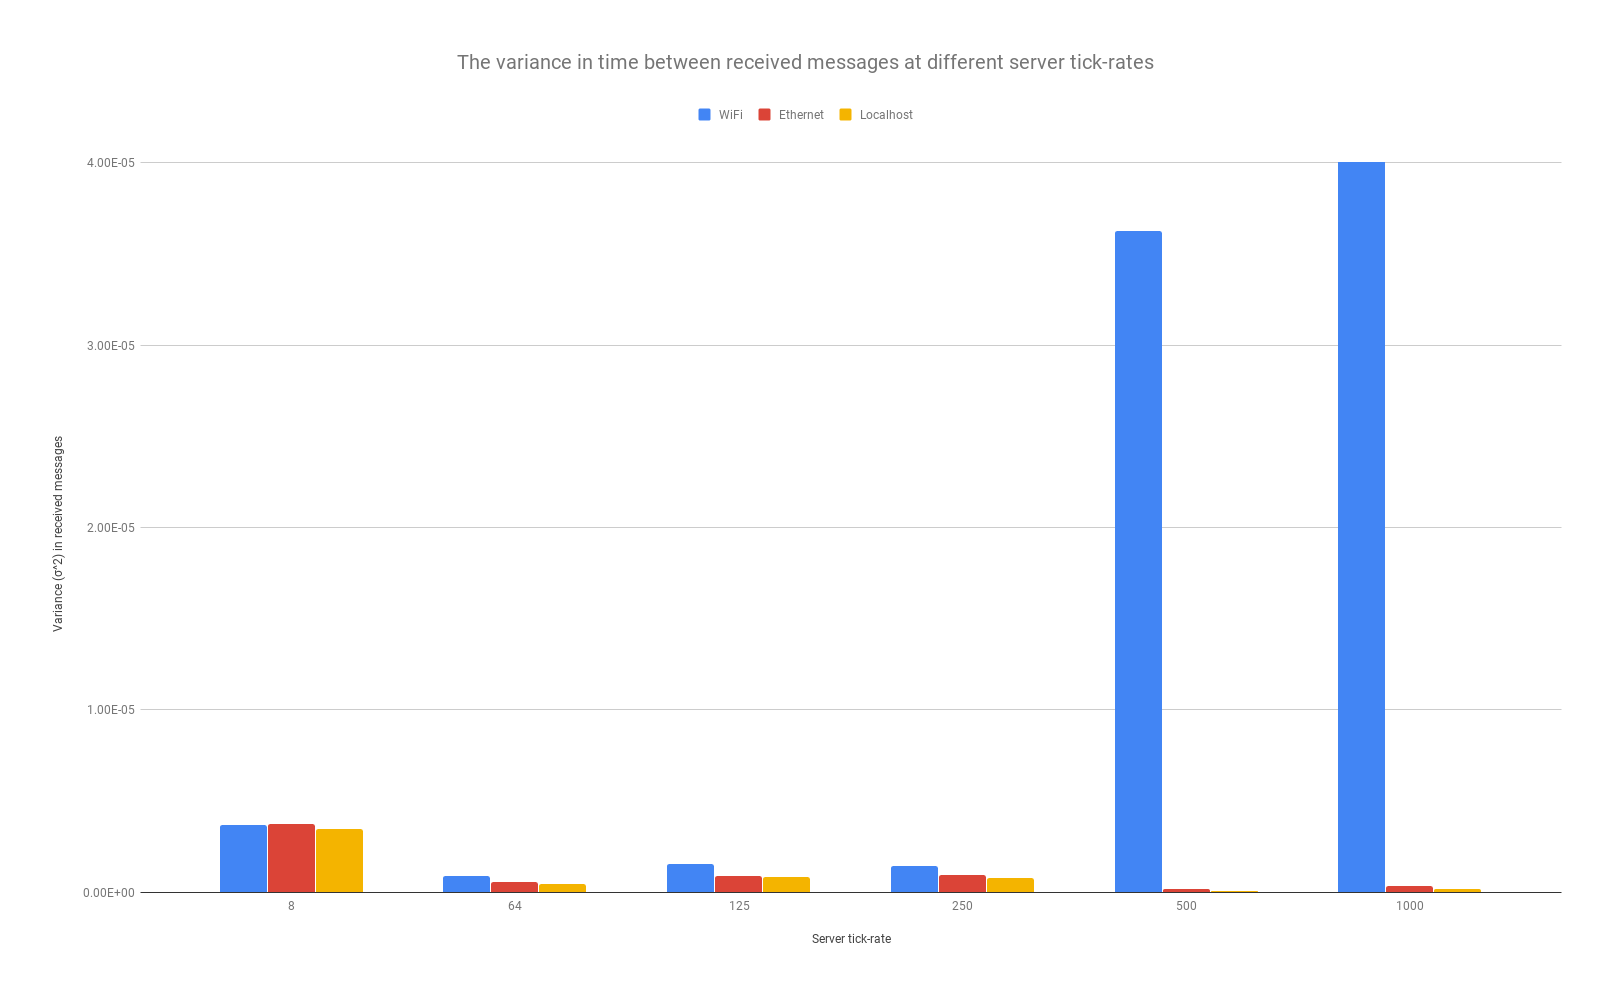
\includegraphics[width=\textwidth]{Graphs/jitter_variance}
  \caption{Graph showing the variance in the delay between receiving messages.}
  \label{fig:jitter_variance}
\end{figure}


\chapter{Conclusion}
